% CS765 Aspects of System Administration
% Author: Jan Schaumann <jschauma@netmeister.org>
% $Id: slides.tex,v 1.7 2004/07/06 20:05:22 jschauma Exp $
\special{! TeXDict begin /landplus90{true}store end }

\documentclass[xga]{xdvislides}
\usepackage[landscape]{geometry}
\usepackage{graphics}
\usepackage{graphicx}
\usepackage{colordvi}

\begin{document}
\setfontphv

%%% Headers and footers
\lhead{\slidetitle}                               % default:\lhead{\slidetitle}
\chead{CS765 - Aspects of System Administration}% default:\chead{\relax}
\rhead{Slide \thepage}                       % default:\rhead{\sectiontitle}
\lfoot{\Gray{System Security}}% default:\lfoot{\slideauthor}
\cfoot{\relax}                               % default:\cfoot{\relax}
\rfoot{\Gray{\today}}
\vspace*{\fill}
\begin{center}
	\Hugesize
		CS615 - Aspects of System Administration\\ [1em]
		System Security\\ [1em]
	\hspace*{5mm}\blueline\\ [1em]
	\Normalsize
		Department of Computer Science\\
		Stevens Institute of Technology\\
		Jan Schaumann\\
		\verb+jschauma@stevens.edu+ \\
		\verb+http://www.cs.stevens.edu/~jschauma/615/+
\end{center}
\vspace*{\fill}

\subsection{Joke Day}
\vspace*{\fill}
\begin{center}
\Huge
WHO HAS ANY ARP JOKES?
\Normalsize
\end{center}
\vspace*{\fill}

\subsection{When is a computer system secure?}
\vspace*{\fill}
\begin{center}
	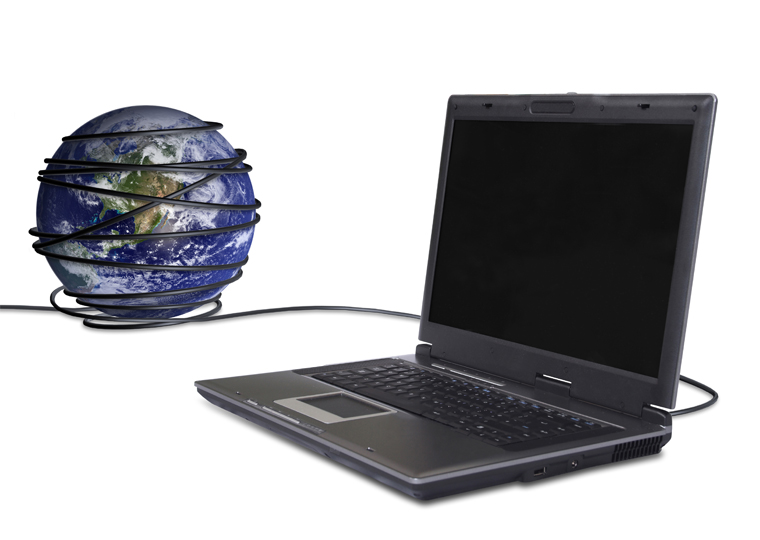
\includegraphics[scale=0.6]{pics/computerwithworld.eps}
\end{center}
\vspace*{\fill}

\subsection{When is a computer system secure?}
\vspace*{\fill}
\begin{center}
	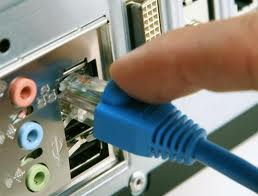
\includegraphics[scale=1.6]{pics/unplug.eps}
\end{center}
\vspace*{\fill}

\subsection{When is a computer system secure?}
\vspace*{\fill}
\begin{center}
	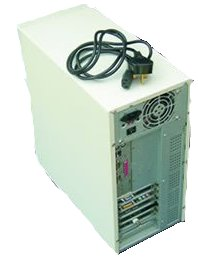
\includegraphics[scale=1.3]{pics/unplugged.eps}
\end{center}
\vspace*{\fill}

\subsection{When is a computer system secure?}
\vspace*{\fill}
\begin{center}
	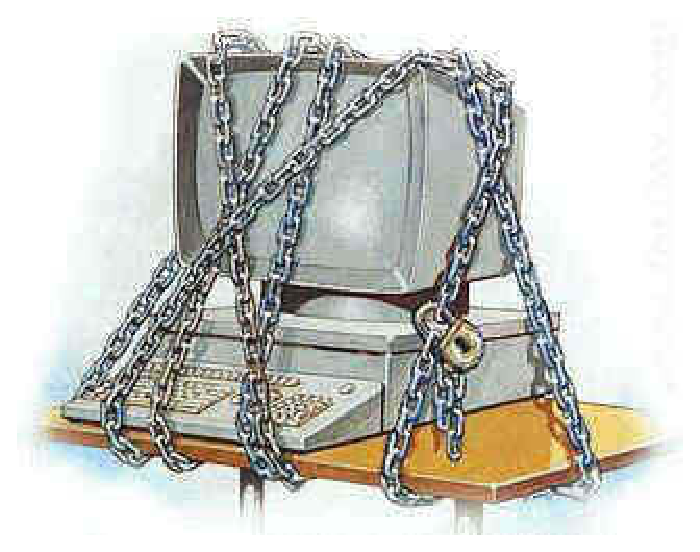
\includegraphics[scale=1.3]{pics/ComputerChainedDown.eps}
\end{center}
\vspace*{\fill}

\subsection{When is a computer system secure?}
\vspace*{\fill}
\begin{center}
	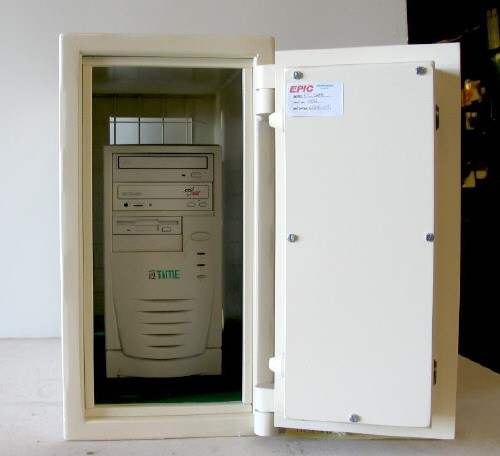
\includegraphics[scale=1.7]{pics/computer_in_safe.eps}
\end{center}
\vspace*{\fill}

\subsection{When is a computer system secure?}
\vspace*{\fill}
\begin{center}
	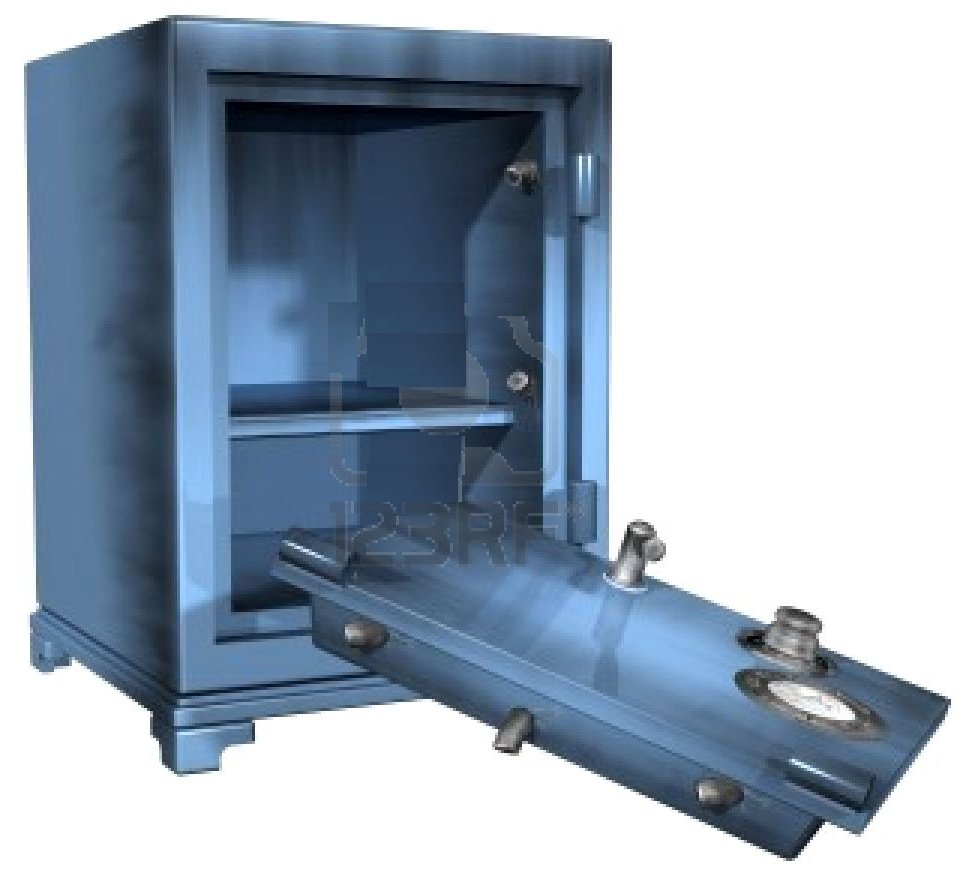
\includegraphics[scale=0.3]{pics/broken-safe.eps}
\end{center}
\vspace*{\fill}

\subsection{When is a computer system secure?}
\vspace*{\fill}
\begin{center}
	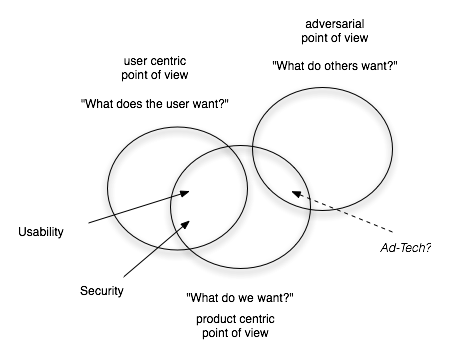
\includegraphics[scale=0.6]{pics/security-usability.eps}
\end{center}
\vspace*{\fill}



\subsection{What is security?}
\Huge
\begin{verbatim}
security

 NOUN:

   Freedom from risk or danger; safety.
\end{verbatim}
\Normalsize

\subsection{What is risk?}
\Huge
\begin{verbatim}
risk

 NOUN:

  The possibility of suffering harm or loss; danger.
\end{verbatim}
\Normalsize

\subsection{What danger are you facing?}
Suffering harm or loss of {\em what}?

\subsection{What danger are you facing?}
Suffering harm or loss of {\em what}?

\begin{itemize}
	\item access to data
\end{itemize}

\subsection{What danger are you facing?}
Suffering harm or loss of {\em what}?

\begin{itemize}
	\item access to data
	\item integrity of data
\end{itemize}

\subsection{What danger are you facing?}
Suffering harm or loss of {\em what}?

\begin{itemize}
	\item access to data
	\item integrity of data
	\item availability of services
\end{itemize}

\subsection{What danger are you facing?}
Suffering harm or loss of {\em what}?

\begin{itemize}
	\item access to data
	\item integrity of data
	\item availability of services
	\item reputation
\end{itemize}

\subsection{What danger are you facing?}
Suffering harm or loss of {\em what}?

\begin{itemize}
	\item access to data
	\item integrity of data
	\item availability of services
	\item reputation
	\item monetary loss due to any of the above
\end{itemize}

\subsection{What danger are you facing?}
Suffering harm or loss of {\em what}?

\begin{itemize}
	\item access to data
	\item integrity of data
	\item availability of services
	\item reputation
	\item monetary loss due to any of the above
	\item monetary loss due to physical items of actual value
\end{itemize}

\subsection{How to determine {\em risk}}
``Risk Assessment''
\begin{itemize}
	\item identify {\em assets}
\end{itemize}

\subsection{How to determine {\em risk}}
``Risk Assessment''
\begin{itemize}
	\item identify {\em assets}
	\item identify {\em threats}
\end{itemize}


\subsection{How to determine {\em risk}}
``Risk Assessment''
\begin{itemize}
	\item identify {\em assets}
	\item identify {\em threats}
	\item identify {\em vulnerabilities}
\end{itemize}

\subsection{How to determine {\em risk}}
``Risk Assessment''
\begin{itemize}
	\item identify {\em assets}
	\item identify {\em threats}
	\item identify {\em vulnerabilities}
	\item determine {\em likelihood of damage}
\end{itemize}

\subsection{How to determine {\em risk}}
``Risk Assessment''
\begin{itemize}
	\item identify {\em assets}
	\item identify {\em threats}
	\item identify {\em vulnerabilities}
	\item determine {\em likelihood of damage}
	\item estimate {\em cost of recovery}
\end{itemize}

\subsection{How to determine {\em risk}}
``Risk Assessment''
\begin{itemize}
	\item identify {\em assets}
	\item identify {\em threats}
	\item identify {\em vulnerabilities}
	\item determine {\em likelihood of damage}
	\item estimate {\em cost of recovery}
	\item estimate {\em cost of defense}
\end{itemize}

\subsection{How to determine {\em risk}}
``Risk Assessment''
\begin{itemize}
	\item identify {\em assets}
	\item identify {\em threats}
	\item identify {\em vulnerabilities}
	\item determine {\em likelihood of damage}
	\item estimate {\em cost of recovery}
	\item estimate {\em cost of defense}
\end{itemize}
\vspace{.5in}

A {\em risk} is the {\em likelihood} of a {\em threat} successfully exploiting
a {\em vulnerability} and the {\em estimated cost} (or potential damage) both
in the short and long term you may incur as a result.

\subsection{Joke Day}
\vspace*{\fill}
\begin{center}
\Huge
I wrote down a Perl joke six months ago, but now I can’t read it.
\Normalsize
\end{center}
\vspace*{\fill}

\subsection{It's not just 1s and 0s}
\vspace{.5in}

\Huge
\begin{center}
System security is not restricted to {\em software} security.
\end{center}
\Normalsize

\subsection{Physical Security}
\vspace{.5in}

\Huge
\begin{center}
If you have even only temporary physical access to a machine, you own it.
\end{center}
\Normalsize

\subsection{Joke Day}
\vspace*{\fill}
\begin{center}
\Huge
There are no bad Apple jokes, you simply tell them wrong.
\Normalsize
\end{center}
\vspace*{\fill}


\subsection{Types of Software Vulnerabilities}
(Distributed) Denial of Service
\begin{center}
	\includegraphics[scale=1.0]{pics/ddos.eps}
\end{center}

\subsection{Types of Software Vulnerabilities}
Privilege Escalation
\begin{center}
	
\includegraphics[scale=0.6]{pics/escalation.eps}
\end{center}

\subsection{Types of Software Vulnerabilities}
Backdoors and Trojans
\begin{center}
	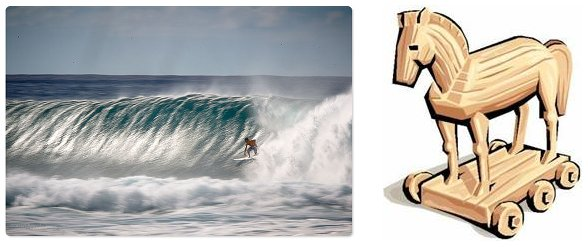
\includegraphics[scale=0.9]{pics/backdoor-trojans.eps}
\end{center}

%\subsection{Types of Software Vulnerabilities}
%Information Disclosure
%\begin{center}
%	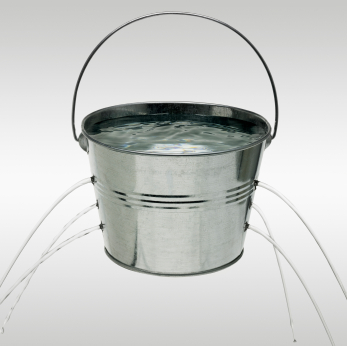
\includegraphics[scale=0.2]{pics/leaking-bucket.eps}
%\end{center}
%
\subsection{Types of Software Vulnerabilities}
Social Engineering (such as phishing)
\begin{center}
	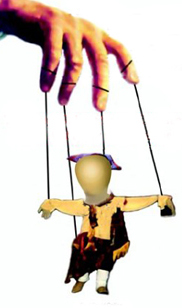
\includegraphics[scale=1.0]{pics/social_engineering.eps}
	
\includegraphics[scale=0.8]{pics/fishing.eps}
\end{center}

\subsection{Types of Software Vulnerabilities}
SQL Injection
\begin{center}
	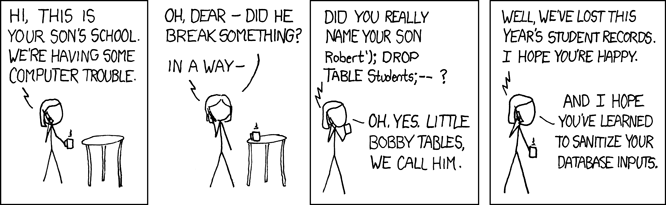
\includegraphics[scale=1.0]{pics/bobby-tables.eps} \\
	\verb+https://xkcd.com/327/+
\end{center}


\subsection{Of course...}
\vspace*{\fill}
\begin{center}
	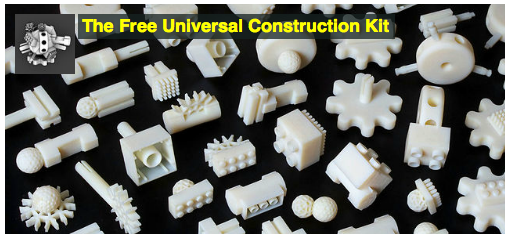
\includegraphics[scale=1.0]{pics/adapters.eps}  \\
	\verb+http://fffff.at/free-universal-construction-kit/+ \\
\end{center}
\vspace*{\fill}

\subsection{Joke Day}
\vspace*{\fill}
\begin{center}
\Huge
The great thing about rsync jokes is that it only tells them if you
haven't heard them before.
\Normalsize
\end{center}
\vspace*{\fill}


\subsection{Encryption}
{\em Encryption} can help mitigate {\em some} of the risks {\em sometimes}.

\subsection{Encryption}
{\em Encryption} can help mitigate {\em some} of the risks {\em sometimes}.
\\

It may provide security in the areas of:
\begin{itemize}
	\item Secrecy or Confidentiality
\end{itemize}

\subsection{Encryption}
{\em Encryption} can help mitigate {\em some} of the risks {\em sometimes}.
\\

It may provide security in the areas of:
\begin{itemize}
	\item Secrecy or Confidentiality
	\item Accuracy or Integrity
\end{itemize}

\subsection{Encryption}
{\em Encryption} can help mitigate {\em some} of the risks {\em sometimes}.
\\

It may provide security in the areas of:
\begin{itemize}
	\item Secrecy or Confidentiality
	\item Accuracy or Integrity
	\item Authenticity
\end{itemize}

\subsection{Encryption}
{\em Encryption} can help mitigate {\em some} of the risks {\em sometimes}.
\\

It may provide security in the areas of:
\begin{itemize}
	\item Secrecy or Confidentiality
		\begin{itemize}
			\item {\em Did/could anybody else see (parts of) the message?}
		\end{itemize}
	\item Accuracy or Integrity
	\item Authenticity
\end{itemize}

\subsection{Encryption}
{\em Encryption} can help mitigate {\em some} of the risks {\em sometimes}.
\\

It may provide security in the areas of:
\begin{itemize}
	\item Secrecy or Confidentiality
		\begin{itemize}
			\item {\em Did/could anybody else see (parts of) the message?}
		\end{itemize}
	\item Accuracy or Integrity
		\begin{itemize}
			\item {\em Was the message (could it have been) modified before I received it?}
		\end{itemize}
	\item Authenticity
\end{itemize}

\subsection{Encryption}
{\em Encryption} can help mitigate {\em some} of the risks {\em sometimes}.
\\

It may provide security in the areas of:
\begin{itemize}
	\item Secrecy or Confidentiality
		\begin{itemize}
			\item {\em Did/could anybody else see (parts of) the message?}
		\end{itemize}
	\item Accuracy or Integrity
		\begin{itemize}
			\item {\em Was the message (could it have been) modified before I received it?}
		\end{itemize}
	\item Authenticity
		\begin{itemize}
			\item {\em Is the party I'm talking to actually
who I think it is / they claim they are?}
		\end{itemize}
\end{itemize}

\subsection{Basic Security Concepts: Confidentiality}
\begin{itemize}
	\item Alice and Bob agree on a way to transform data
	\item transformed data is sent over insecure channel
	\item Alice and Bob are able to get data out of the transformation
\end{itemize}
\addvspace{.5in}
\begin{verbatim}
$ cat secret
Oehpr Fpuarvre rkcrpgf gur Fcnavfu Vadhvfvgvba!
$
\end{verbatim}

\subsection{Basic Security Concepts: Confidentiality}
\begin{itemize}
	\item Alice and Bob agree on a way to transform data
	\item transformed data is sent over insecure channel
	\item Alice and Bob are able to get data out of the transformation
\end{itemize}
\addvspace{.5in}
\begin{verbatim}
$ cat secret
Oehpr Fpuarvre rkcrpgf gur Fcnavfu Vadhvfvgvba!
$ cat secret | rot13
Bruce Schneier expects the Spanish Inquisition!
$
\end{verbatim}

%\subsection{Basic Security Concepts: Confidentiality}
%\begin{itemize}
%	\item Alice and Bob agree on a way to transform data
%	\item transformed data is sent over insecure channel
%	\item Alice and Bob are able to get data out of the transformation
%\end{itemize}
%\addvspace{.5in}
%\begin{verbatim}
%$ cat secret
%Jrbk.pycbi x.y,..b ekrpat abe ',.pyf jab ugbjycrb ao a ocmln. ogxoycygycrb jfld.p!
%$ cat secret | qibenx2djregl
%[...]
%$
%\end{verbatim}
%
\subsection{Basic Security Concepts: Confidentiality}
\begin{itemize}
	\item Alice and Bob agree on a way to transform data
	\item transformed data is sent over insecure channel
	\item Alice and Bob are able to get data out of the transformation
\end{itemize}
\addvspace{.5in}
\begin{center}
	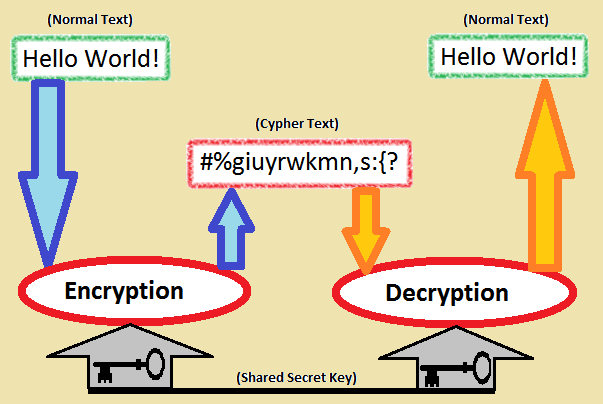
\includegraphics[scale=0.75]{pics/symmetric-key-crypto.eps}
\end{center}

\subsection{Basic Security Concepts: Confidentiality}
Different approaches:
\begin{itemize}
	\item secret key cryptography (example: {\em DES})
		\begin{itemize}
			\item Alice and Bob share a secret
			\item Alice can prove to Bob that she knows a secret
		\end{itemize}
\end{itemize}
 \begin{center}
        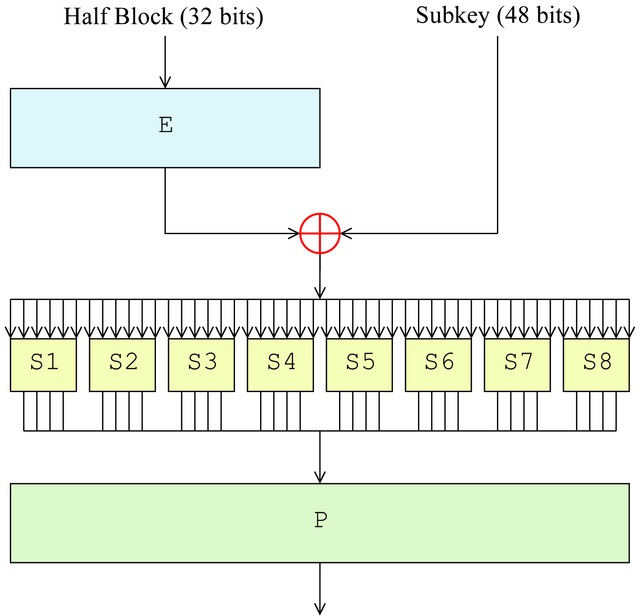
\includegraphics[scale=0.42]{pics/DES-f-function.eps} \\
 \end{center}

\subsection{Basic Security Concepts: Confidentiality}
Different approaches:
\begin{itemize}
	\item public key cryptography (example: {\em RSA})
		\begin{itemize}
			\item Alice has a private and a public key
			\item data encrypted with her private key can only be decrypted by
				her public key and vice versa
			\item public key can be shared with anybody (via insecure means)
		\end{itemize}
\end{itemize}
\begin{center}
	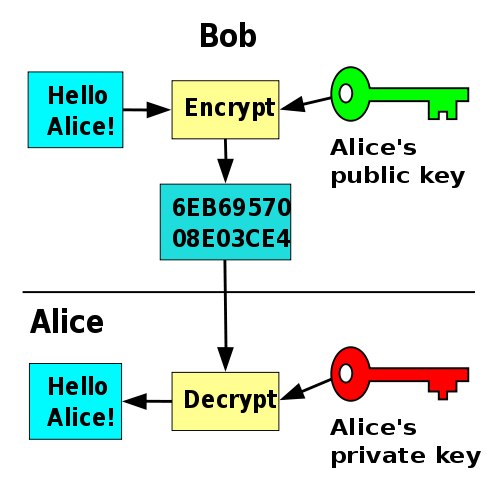
\includegraphics[scale=0.43]{pics/Public_key_encryption.eps}
 \end{center}

\subsection{Basic Security Concepts: Integrity}
In order to protect against forgery or data manipulation, provide some sort of
digest or checksum (often a one-way hash).  Popular choices:

\begin{itemize}
	\item {\tt 5f4dcc3b5aa765d61d8327deb882cf99}
	\item {\tt 5baa61e4c9b93f3f0682250b6cf8331b7ee68fd8}
	\item {\tt 5e884898da28047151d0e56f8dc6292773603d0d6aabbdd62 \
                   a11ef721d1542d8}
	\item {\tt b109f3bbbc244eb82441917ed06d618b9008dd09b3befd1b5 \
                   e07394c706a8bb980b1d7785e5976ec049b46df5f1326af5a \
                   2ea6d103fd07c95385ffab0cacbc86}
\end{itemize}

\subsection{Basic Security Concepts: Integrity}
In order to protect against forgery or data manipulation, provide some sort of
digest or checksum (often a one-way hash).  Popular choices:

\begin{itemize}
	\item {\tt 5f4dcc3b5aa765d61d8327deb882cf99} (MD5)
	\item {\tt 5baa61e4c9b93f3f0682250b6cf8331b7ee68fd8} (SHA-1)
	\item {\tt 5e884898da28047151d0e56f8dc6292773603d0d6aabbdd62 \
                   a11ef721d1542d8} (SHA256)
	\item {\tt b109f3bbbc244eb82441917ed06d618b9008dd09b3befd1b5 \
                   e07394c706a8bb980b1d7785e5976ec049b46df5f1326af5a \
                   2ea6d103fd07c95385ffab0cacbc86} (SHA512)
\end{itemize}

\subsection{Basic Security Concepts: Integrity}
In order to protect against forgery or data manipulation, provide some sort of
digest or checksum (often a one-way hash).  Popular choices:

\begin{itemize}
	\item {\tt 5f4dcc3b5aa765d61d8327deb882cf99} (MD5)
	\item {\tt 5baa61e4c9b93f3f0682250b6cf8331b7ee68fd8} (SHA-1)
	\item {\tt 5e884898da28047151d0e56f8dc6292773603d0d6aabbdd62 \
                   a11ef721d1542d8} (SHA256)
	\item {\tt b109f3bbbc244eb82441917ed06d618b9008dd09b3befd1b5 \
                   e07394c706a8bb980b1d7785e5976ec049b46df5f1326af5a \
                   2ea6d103fd07c95385ffab0cacbc86} (SHA512)
\end{itemize}


Caveats:
\begin{itemize}
	\item ``rainbow tables'' / internet search engines allow for easy reverse
		lookup of un-salted hashes.
	\item integrity only ensured if authenticity of information itself is
		guaranteed
\end{itemize}

\subsection{Basic Security Concepts: Authenticity}
Three general ways of proving that you are who you say you are:
\begin{itemize}
	\item something you know
	\item something you have
	\item something you are
\end{itemize}

\subsection{Basic Security Concepts: Authenticity}
Three general ways of proving that you are who you say you are:
\begin{itemize}
	\item something you know
		\begin{itemize}
			\item secret handshake, password
			\item can (easily) be given to and used by somebody else
		\end{itemize}
	\item something you have
	\item something you are
\end{itemize}

\subsection{Basic Security Concepts: Authenticity}
Three general ways of proving that you are who you say you are:
\begin{itemize}
	\item something you know
		\begin{itemize}
			\item secret handshake, password
			\item can (easily) be given to and used by somebody else
		\end{itemize}
	\item something you have
		\begin{itemize}
			\item physical items: smart card, RSA token, ...
			\item private keys
			\item can (easily) be given to and used by somebody else
		\end{itemize}
	\item something you are
\end{itemize}

\subsection{Basic Security Concepts: Authenticity}
Three general ways of proving that you are who you say you are:
\begin{itemize}
	\item something you know
		\begin{itemize}
			\item secret handshake, password
			\item can (easily) be given to and used by somebody else
		\end{itemize}
	\item something you have
		\begin{itemize}
			\item physical items: smart card, RSA token, ...
			\item private keys
			\item can (easily) be given to and used by somebody else
		\end{itemize}
	\item something you are
		\begin{itemize}
			\item physical, physiological or behavioral traits
			\item can not (easily or at all) be given to or
				used by somebody else
		\end{itemize}
\end{itemize}



\subsection{Basic Security Concepts: Proving Authenticity}
\begin{itemize}
	\item in private key cryptography, authenticity is (often) assumed/implied
	\item in public key cryptography, often accomplished via a separate
		signature
	\item ways to establish assurance of authenticity for parties that have
		never met:
		\begin{itemize}
			\item public key infrastructures (PKI) and certificate
				authorities (CA)
			\item ``web of trust''
		\end{itemize}
\end{itemize}

%\subsection{Basic Security Concepts: PKI}
%\vspace*{\fill}
%\begin{center}
%	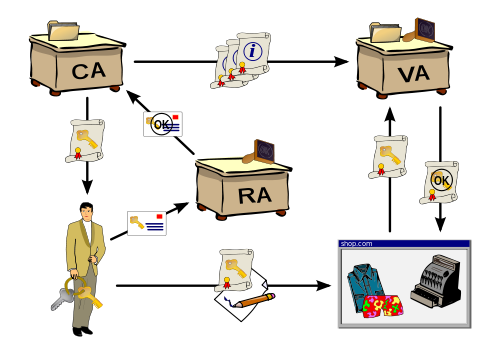
\includegraphics[scale=0.55]{pics/pki.eps}
%\end{center}
%\vspace*{\fill}
%
%\subsection{Basic Security Concepts: Web of Trust}
%\begin{center}
%	\includegraphics[scale=0.6]{pics/belushi-bacon1.eps}
%\end{center}
%\subsection{Basic Security Concepts: Web of Trust}
%\small
%John Belushi, Donald Sutherland (Animal House)
%\begin{center}
%	\includegraphics[scale=0.6]{pics/belushi-bacon2.eps}
%\end{center}
%
%\subsection{Basic Security Concepts: Web of Trust}
%\small
%Donald Sutherland, Pauly Shore (Lost Angels)
%\begin{center}
%	\includegraphics[scale=0.6]{pics/belushi-bacon3.eps}
%\end{center}
%
%\subsection{Basic Security Concepts: Web of Trust}
%\small
%Pauly Shore, Andy Dick (In the Army now)
%\begin{center}
%	\includegraphics[scale=0.6]{pics/belushi-bacon4.eps}
%\end{center}
%
%\subsection{Basic Security Concepts: Web of Trust}
%\small
%Andy Dick, Claudia Schiffer (Zoolander)
%\begin{center}
%	\includegraphics[scale=0.6]{pics/belushi-bacon5.eps}
%\end{center}
%
%\subsection{Basic Security Concepts: Web of Trust}
%\small
%Claudia Schiffer, Sarah Jessica Parker (Life without Dick)
%\begin{center}
%	\includegraphics[scale=0.6]{pics/belushi-bacon6.eps}
%\end{center}
%
%\subsection{Basic Security Concepts: Web of Trust}
%\small
%Sarah Jessica Parker, Kevin Bacon (Footloose)
%\begin{center}
%	\includegraphics[scale=0.6]{pics/belushi-bacon6.eps}
%\end{center}
%\Normalsize
%
%\subsection{Basic Security Concepts: Web of Trust}
%Problems with the Web of Trust:
%\begin{center}
%	\includegraphics[scale=0.8]{pics/pauly-shore.eps}
%	\hspace*{15mm}
%	\includegraphics[scale=1.0]{pics/andy0dick.eps}
%\end{center}
%
%\subsection{Basic Security Concepts: Web of Trust}
%Better:
%\begin{center}
%	\includegraphics[scale=0.8]{pics/bacon-belushi.eps}
%\end{center}
%
%\subsection{Basic Security Concepts: Web of Trust}
%\begin{itemize}
%	\item you have to trust every signing entity in your trustpath
%	\item the shorter the trustpath, the better
%	\item the more nodes, the better
%	\item the more edges, the better
%	\item the fewer leaves, the better
%	\item the more signatures a key has, the better
%\end{itemize}
%

\subsection{Joke Day}
\vspace*{\fill}
\begin{center}
\Huge
I'll keep telling this TCP joke until you get it.
\Normalsize
\end{center}
\vspace*{\fill}


\newpage
\vspace*{\fill}
\begin{center}
    \Hugesize
        Hooray! \\ [1em]
    \hspace*{5mm}
    \blueline\\
    \hspace*{5mm}\\
        5 Minute Break
\end{center}
\vspace*{\fill}


\subsection{Understanding your realistic threats}
\vspace*{\fill}
\begin{center}
	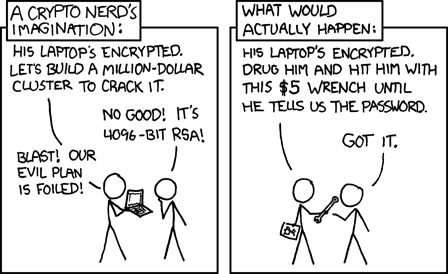
\includegraphics[scale=1.3]{pics/security.eps}
\end{center}
\vspace*{\fill}


\subsection{Some Words of Wisdom}
Bruce Schneier:
\\

\Huge
\begin{center}
Complexity is the worst enemy of security.
\end{center}
\Normalsize

\subsection{Some Words of Wisdom}
Bruce Schneier:
\\

\Huge
\begin{center}
Complexity is the worst enemy of security.
\\
\addvspace{.5in}
The more secure you make something, the less secure it becomes.
\end{center}
\Normalsize

\subsection{Joke Day}
\vspace*{\fill}
\begin{center}
\Huge
The best part about a CISSP joke, is you don't have to know anything about
security to get it.
\Normalsize
\end{center}
\vspace*{\fill}



\subsection{A practical example}
CVE-2006-3555
\\

``The TLS protocol, and the SSL protocol 3.0 and possibly earlier, as used in
Microsoft Internet Information Services (IIS) 7.0, mod\_ssl in the Apache HTTP
Server 2.2.14 and earlier, OpenSSL before 0.9.8l, GnuTLS 2.8.5 and earlier,
Mozilla Network Security Services (NSS) 3.12.4 and earlier, multiple Cisco
products, and other products, does not properly associate renegotiation
handshakes with an existing connection, which allows man-in-the-middle
attackers to insert data into HTTPS sessions, and possibly other types of
sessions protected by TLS or SSL, by sending an unauthenticated request that
is processed retroactively by a server in a post-renegotiation context,
related to a "plaintext injection" attack''
\vspace*{\fill}

\subsection{TLS Renegotation Attack}
\begin{itemize}
	\item TLS allows for ``re-negotation'' {\em within} the existing TLS
		connection
\end{itemize}

\subsection{TLS Renegotation Attack}
\begin{itemize}
	\item TLS allows for ``re-negotation'' {\em within} the existing TLS
		connection
	\item MitM {\em cannot} get plain text from cypher text
\end{itemize}

\subsection{TLS Renegotation Attack}
\begin{itemize}
	\item TLS allows for ``re-negotation'' {\em within} the existing TLS
		connection
	\item MitM {\em cannot} get plain text from cypher text
	\item MitM may be able to inject plain text into encrypted connection
\end{itemize}

\subsection{TLS Renegotation Attack}
\begin{itemize}
	\item TLS allows for ``re-negotation'' {\em within} the existing TLS
		connection
	\item MitM {\em cannot} get plain text from cypher text
	\item MitM may be able to inject plain text into encrypted connection
	\item a clever MitM can either cause unauthorized actions to be performed
		or even cause information disclosure
\end{itemize}

\subsection{TLS Renegotation Attack}
\begin{itemize}
	\item TLS allows for ``re-negotation'' {\em within} the existing TLS
		connection
	\item MitM {\em cannot} get plain text from cypher text
	\item MitM may be able to inject plain text into encrypted connection
	\item a clever MitM can either cause unauthorized actions to be performed
		or even cause information disclosure
\end{itemize}
\addvspace{.5in}

\begin{itemize}
	\item initially dismissed as too academic or theoretical to be practical
\end{itemize}

\subsection{TLS Renegotation Attack}
\begin{itemize}
	\item TLS allows for ``re-negotation'' {\em within} the existing TLS
		connection
	\item MitM {\em cannot} get plain text from cypher text
	\item MitM may be able to inject plain text into encrypted connection
	\item a clever MitM can either cause unauthorized actions to be performed
		or even cause information disclosure
\end{itemize}
\addvspace{.5in}

\begin{itemize}
	\item initially dismissed as too academic or theoretical to be practical
	\item until Twitter was hit and users' accounts were broken into using
		precisely this vulnerability
\end{itemize}

\subsection{Joke Day}
\vspace*{\fill}
\begin{center}
\Huge
There are 10 types of people in the world: Those who understand binary,
and those who don't.
\Normalsize
\end{center}
\vspace*{\fill}


\subsection{Whom do you trust?}
\begin{center}
	
\includegraphics[scale=1.0]{pics/sledgehammer.eps}
\end{center}

\subsection{Further Reflections on Trust}
Compromised EC2 image includes root access SSH key -
{\tt http://pastebin.com/q1VH4rmF}
\\

Intentional? Malicious? Accidental?
\\

Does it matter?

\subsection{Outsourcing Services}
\begin{itemize}
	\item you trust the provider/vendor to honor the agreement
	\item you ``hope'' they won't change their agreement (once
		invested, changing back is hard)
	\item you trust the provider/vendor to keep their infrastructure
		safe
	\item you are ok with the traffic going across the public internet
\end{itemize}

\subsection{Outsourcing Services}
\begin{itemize}
	\item you trust the provider/vendor to honor the agreement
	\item you ``hope'' they won't change their agreement (once
		invested, changing back is hard)
	\item you trust the provider/vendor to keep their infrastructure
		safe
	\item you are ok with the traffic going across the public internet
\end{itemize}
\vspace{.5in}

Note: in some cases, outsourcing happens one way or another (gmail,
anybody?).


\subsection{Toning down the Paranoia}
Hanlon's Razor:
\\

\Huge
\begin{center}
Never attribute to malice that which can be adequately explained by stupidity.
\end{center}
\Normalsize

\subsection{Toning down the Paranoia}
Sturgeon's Law (first adage):
\\

\Huge
\begin{center}
Nothing is always absolutely so.
\end{center}
\Normalsize


\subsection{What to do in the case of an emergency}

As usual, this {\em depends}.  Some the smarter things to do if you detect an
intrusion include:

\begin{itemize}
	\item keep system online to monitor what the attacker does or how she
		gained access, {\em or}
	\item take system offline, possible entirely into single user mode
	\item take a complete snapshot of the system to separate media
	\item keep system offline while you investigate
	\item reinstall
\end{itemize}

Remember that you can't trust {\em any} data on the compromised system!

\subsection{Miscellaneous}
Things probably mentioned before, but worth repeating:
\begin{itemize}
	\item subscribe to your vendors security alert mailinglist
	\item subscribe to independent security alert mailinglists
	\item checksum and verify any and all packages and patches
	\item regularly audit the installed software
	\item require strong passwords
	\item inform your users of security issues
	\item guard against threats from outside as well as inside the network
		(ie revisit whom you think you can trust)
\end{itemize}

\subsection{Joke Day}
\vspace*{\fill}
\begin{center}
\Huge
The problem with 802.11 jokes is they probably go over your head.
\Normalsize
\end{center}
\vspace*{\fill}



\subsection{Be Paranoid!}
\begin{center}
	
\includegraphics[scale=0.55]{pics/paranoid.eps}
\end{center}

\subsection{Reading}
TLS MitM attack:
\\

\verb+http://www.securegoose.org/2009/11/tls-renegotiation-vulnerability-cve.html+ \\

\verb+http://www.educatedguesswork.org/2009/11/understanding_the_tls_renegoti.html+
\Normalsize

\subsection{Reading}
Helpful Tools:
\begin{itemize}
	\item \verb+mtree(1)+
	\item \verb+gpg(1)+
\end{itemize}
\addvspace{.5in}
Helpful Information:
\begin{itemize}
	\item CSRC NIST \verb+http://csrc.nist.gov/+
	\item SecurityFocus \verb+http://www.securityfocus.com/+
	\item CryptoGram \verb+http://www.counterpane.com/crypto-gram.html+
\end{itemize}
\addvspace{.5in}
Misc:
\\

\verb+http://archive.cert.uni-stuttgart.de/isn/2006/01/msg00055.html+
\\

\verb+http://is.gd/p9Q0pU+

\end{document}
